\section{Theory}
\subsection{IRMA}
Here we explain the background of the IRMA proofs.

\subsubsection{Usage scenario}
Beschrijven hoe de basic course of events verloopt, en welke voorwaarden daarbij gelden. Denk aan het veilig opbergen van tablet in kluis, wellicht pincode op tablet, etc.

\subsection{Passport}
The passport is a travel document issued by a country's government that certifies the identity and nationality of its holder for the purpose of international travel~\cite{passportdefinition}. A biometric passport is an upgraded version that contains biometric information that can be used to authenticate the identity of travelers. This information is stored on an embedded chip that can be read using contactless smart card technology. Passports that feature such a chip generally feature the symbol shown in figure~\ref{fig:biometricslogo} on the cover. The data stored on the passport chip needs to be protected from modification, cloning, eavesdropping, etc. For this purpose several protection mechanisms have been implemented. Each of these mechanisms exist alongside each other and protect against different types of attacks. This section describes the various security protocols supported by passports, i.e. PA, BAC, SM and AA as specified by ICAO in~\cite{icao} as well as EAC as specified in~\cite{bsi}. 

\begin{figure}[htb]
	\centering
		
\includegraphics{images/biometrics_logo.svg}
	\caption{Symbol to indicate a biometric passport}
	\label{fig:biometricslogo}
\end{figure}

\subsubsection{Passive Authentication}
Passive Authentication (PA) is not actually a protocol. It simply indicates that the chip makes use of digital signatures of its data. PA involves the terminal reading the data and verifying both its hash and signature. PA is the only `protocol' that is mandatory; all other protocols are optional~\cite{mostowski2010electronic}.

\subsubsection{Basic Access Control}
Consider the case where a passport does not feature an RF chip. In this scenario privacy of the passport data is achieved by being able to keep the passport closed so nobody can read its data. With the addition of the RF chip this would no longer hold. Anyone with an RF reader (often called a terminal) is able to read the data on the chip if it is in close proximity. The solution to this problem is to protect the data with a key that the reader needs to know before being allowed to read the data. This is how the Basic Access Control (BAC) protocol works. BAC is essentially not required to be used by ePassports, but is strongly recommended. The key used for BAC is derived from three properties of the passport.
\begin{enumerate}
	\item The document number (usually 9 digits)
  \item The date of birth (formatted YYMMDD in Dutch passports)
  \item The document expiry date (formatted YYMMDD in Dutch passports)
\end{enumerate}
These three properties are part of the Machine Readable Zone (MRZ) that is printed in monospace at the bottom of the passport (see figure~\ref{fig:dutchpassport}). Also part of the MRZ is the Burger Service Nummer (BSN), which uniquely identifies a Dutch citizen, but this number is not used for the key derivation for BAC. Combining the aforementioned properties eventually results in the key with which the reader may access the chip's data. Keep in mind the MRZ is not visible while the passport is closed and cannot be obtained anywhere else. The only method of transferring the MRZ to the reader is for the reader to either utilize optical character recognition (OCR) software or for the passport holder to manually enter the information into the reader. In either case the MRZ is transmitted via an out of band channel. After the key is used for authenticating the reader to the passport, all further communication is performed via an encrypted channel~\cite{icao}.

In some countries, e.g. the US, the chip is shielded by a very thin metal mesh that is integrated into the cover of the passport. This prevents readers from accessing the chip without having the passport holder open his or her passport first.[citation needed]~\footnote{\url{https://www.newscientist.com/article/dn8227-metal-shields-and-encryption-for-us-passports/}}.

\textsc{Supplemental Access Control (SAC) was introduced by ICAO in 2009 for addressing BAC weaknesses. It was introduced as a supplement to BAC (for keeping compatibility), but will replace it in the future.} It is mandatory from December 2014 onwards\footnote{\url{http://www.securitydocumentworld.com/creo_files/upload/client_files/moving_to_the_third_generation_of_electronic_passports_october_20111.pdf}}

\begin{figure}[htb]
	\centering
		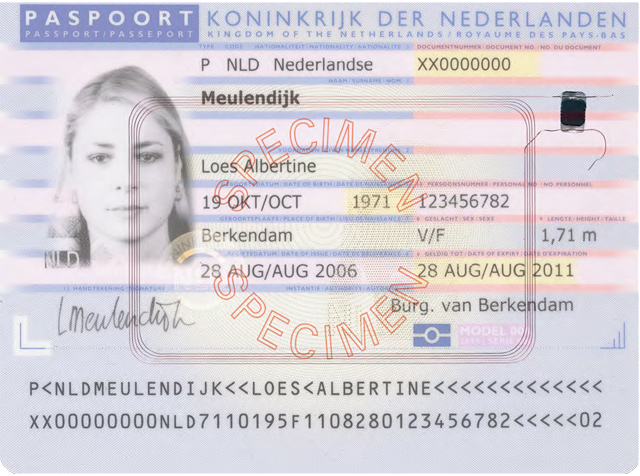
\includegraphics[width=0.50\textwidth]{images/dutchpassport.png}
	\caption{Example of a Dutch passport including a Machine Readable Zone}
	\label{fig:dutchpassport}
\end{figure}

\subsubsection{Secure Messaging}
The Secure Messaging (SM) protocol is used to protect the integrity and confidentiality of the communication between terminal and chip. Essentially the protocol sets up a secure channel, the key for which is agreed upon during the BAC protocol. When also performing EAC, the CA part will refresh the key (see below).

\subsubsection{Extended Access Control}
Starting in 2006 many countries added their citizens' finger prints and iris scans to the chip, by definition turning it into a biometric passport. The biometric data is a lot more sensitive than the data protected by BAC, meaning it needs to be protected by stronger cryptography. For this the Extended Access Control (EAC) protocol was developed and added to the second generation of ePassports in 2009\footnote{\url{http://www.securitydocumentworld.com/creo_files/upload/client_files/moving_to_the_third_generation_of_electronic_passports_october_20111.pdf}}. Any reader that has successfully performed BAC may subsequently perform EAC in order to obtain access to the finger print and iris of the passport holder. EAC is implemented in all new generation EU passports.

EAC consists of two protocols, Chip Authentication (CA) and Terminal Authentication (TA), both relying on a public key infrastructure (PKI) in which certificates are issued to the passport as well as other governments for verification purposes. The CA protocol is used for the terminal to authenticate the chip. It is based on a secret key agreement and a successful run of the protocol provides both parties with a new key for SM. The TA protocol is used for authenticating the terminal to the chip and possibly increase access rights. It actively verifies certificates. After both protocols have finished, mutual authentication is achieved and a new secure channel is created.


\subsubsection{Active Authentication}
\textsc{Active Authentication (AA). AA prevents cloning of passport chips. The chip contains a private key that cannot be read or copied, but its existence can easily be proven. Using AA is optional.}

Active Authentication (AA) is a challenge-response protocol that proves the authenticity of the chip, verifying the chip has not been cloned. The chip contains a private key, of which the chip proves knowledge during AA, and a certificate for this key as signed by the passport issuing country. This protocol is redundant when the passport also supports EAC, since the CA protocol also (implicitly) proves knowledge of this private key. This means that AA is only useful in cases where passports do not support EAC, but still wish to verify knowledge of the private key.

\textsc{Text below copied from Wikipedia: \url{https://en.wikipedia.org/wiki/Biometric_passport}} 

Since the introduction of biometric passports several attacks have been presented and demonstrated:

\begin{itemize}
	\item Non-traceable chip characteristics. In 2008 a Radboud/Lausitz University team demonstrated that it's possible to determine which country a passport chip is from without knowing the key required for reading it.[7] The team fingerprinted error messages of passport chips from different countries. The resulting lookup table allows an attacker to determine from where a chip originated. In 2010 Tom Chothia and Vitaliy Smirnov documented an attack that allows an individual passport to be traced,[8][9] by sending specific BAC authentication requests.
  \item Basic Access Control (BAC). In 2005 Marc Witteman showed that the document numbers of Dutch passports were predictable,[10] allowing an attacker to guess/crack the key required for reading the chip. In 2006 Adam Laurie wrote software that tries all known passport keys within a given range, thus implementing one of Witteman's attacks. Using online flight booking sites, flight coupons and other public information it's possible to significantly reduce the number of possible keys. Laurie demonstrated the attack by reading the passport chip of a Daily Mail's reporter in its envelope without opening it.[11] Note that in some early biometric passports BAC wasn't used at all, allowing attacker to read the chip's content without providing a key.[12]
  \item Passive Authentication (PA). In 2006 Lukas Grunwald demonstrated that it is trivial to copy passport data from a passport chip into a standard ISO/IEC 14443 smartcard using a standard contactless card interface and a simple file transfer tool.[13] Grunwald used a passport that did not use Active Authentication (anti-cloning) and did not change the data held on the copied chip, thus keeping its cryptographic signature valid. In 2008 Jeroen van Beek demonstrated that not all passport inspection systems check the cryptographic signature of a passport chip. For his demonstration Van Beek altered chip information and signed it using his own document signing key of a non-existing country. This can only be detected by checking the country signing keys that are used to sign the document signing keys. To check country signing keys the ICAO PKD[14] can be used. Only 5 out of 60+ countries are using this central database.[15] Van Beek did not update the original passport chip: instead an ePassport emulator was used.[16] Also in 2008, The Hacker's Choice implemented all attacks and published code to verify the results.[17] The release included a video clip that demonstrated problems by using a forged Elvis Presley passport that is recognized as a valid US passport.[18][19]
  \item Active Authentication (AA). In 2005 Marc Witteman showed that the secret Active Authentication key can be retrieved using power analysis.[10] This may allow an attacker to clone passport chips that use the optional Active Authentication anti-cloning mechanism on chips – if the chip design is susceptible to this attack. In 2008 Jeroen van Beek demonstrated that optional security mechanisms can be disabled by removing their presence from the passport index file.[20] This allows an attacker to remove – amongst others – anti-cloning mechanisms (Active Authentication). The attack is documented in supplement 7 of Doc 9303 (R1-p1\_v2\_sIV\_0006)[21] and can be solved by patching inspection system software. Note that supplement 7 features vulnerable examples in the same document that – when implemented – result in a vulnerable inspection process.
  \item Extended Access Control (EAC). In 2007 Luks Grunwald presented an attack that can make EAC-enabled passport chips unusable.[22] Grunwald states that if an EAC-key – required for reading fingerprints and updating certificates – is stolen or compromised, an attacker can upload a false certificate with an issue date far in the future. The affected chips block read access until the future date is reached.
\end{itemize}



Example: active authentication in e-passport
\begin{itemize}
	\item private key securely embedded in passport chip
  \item public key signed by producer (Morpho in NL)
  \item Morpho's public key signed by Dutch state
\end{itemize}
